% Problem ID: 057
% Original file: Training_1/contents/area.tex

\numbering 사각형 $ABCD$ 에서 각 변의 중점을 이어서 만든 사각형의 넓이를 각각
$S_1, S_2, S_3, S_4$ 라 하면 
\[ S_1 + S_3 = S_2 + S_4 \]
가 성립함을 보여라.
\begin{center}
\resizebox{5cm}{5cm}{%
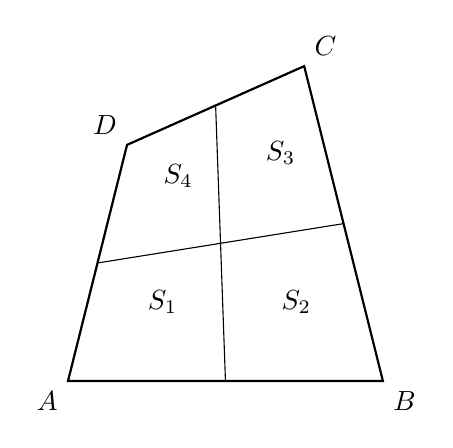
\begin{tikzpicture} 
	\draw[thick] (-2,-2) node[below left] {$A$} 
		-- (2, -2) node[below right] {$B$}
		-- (1, 2) node[above right] {$C$}
		-- (-1.25, 1) node[above left] {$D$} -- cycle ; 
		
	\draw[thin] (0, -2) -- ( {(1-1.25)/2}, {(1+2)/2} )		
			( 1.5, 0) -- ({(-2-1.25)/2}, -0.5);
			
	\draw (-0.8,-1) node {$S_1$} (0.9, -1) node {$S_2$} ;
	\draw (0.7, 0.9) node {$S_3$} (-0.6, 0.6) node {$S_4$} ;
\end{tikzpicture}
}
\end{center}